\chapter{Những trường hợp đặc biệt}

\section{Liên hệ với xích Markov}

\subsection{Xích Markov}
Xích Markov là mô hình toán học mô tả quá trình chuyển dịch từ một trạng thái sang một trạng thái khác dựa trên một số quy luật xác suất nhất định. Trong quá trình đó, xích Markov không quan tâm đến thông tin của quá trình dẫn đến trạng thái hiện tại, mà xác suất của trạng thái tiếp theo chỉ phụ thuộc vào trạng thái hiện tại và xác suất đang có tại thời điểm $t$.\\[10pt]
\textbf{Chúng ta định nghĩa xích Markov là đối tượng toán học trừu tượng bao gồm:} 
\begin{itemize}
    \item Bộ những trạng thái $X$.
    \item Ma trận chuyển trạng thái $P$ với $P_{ij} = P (X_t = i, X_{t-1} =j)$.
    \item $\pi$ là chỉ định phân phối xác suất cố định của mỗi trạng thái $x \in X$.
    \item Mục tiêu tìm ra $\pi = P \pi$.
\end{itemize}
\textbf{Định lý cơ bản của xích Markov:} Với bất kỳ vector nào, phép lặp luỹ thừa được áp dụng cho ma trận chuyển trạng thái $M$ sẽ hội tụ thành một vector dương, tĩnh và duy nhất nếu đồ thị của nó thoả mãn 3 thuộc tính: \emph{stochastic}, \emph{irreducible}, \emph{aperiodic}.
\begin{itemize}
    \item Một đồ thị thoả mãn tính chất \textit{stochastic} nếu ma trận biểu diễn nó có tổng mỗi cột hoặc hàng bằng 1. 
    \item Một đồ thị gọi là \emph{irreducible} nếu đồ thị của nó biểu diễn 1 đồ thị liên thông mạnh.
    \item  Một quá trình là \emph{periodic} nếu tồn tại ít nhất một trạng thái mà quá trình sẽ trả về trạng thái đó sau một khoảng thời gian cố định (lớn hơn 1). Aperiodic nghĩa là không tồn tại trạng thái nào như vậy cả.
\end{itemize}

\subsection{Áp dụng vào PageRank}
%\textbf{Diễn giải PageRank dưới dạng xích Markov:}\\
Mỗi trang web hay mỗi node trong \emph{web graph} có thể xem như một trạng thái. Tại mỗi trang web $i$ có $d^+(i)$ \emph{outgoing links}. Với xác suất mà chúng ta chuyển sang trang web khác là là $\dfrac{1}{d^+(i)}$. Bây giờ chúng ta có thể diễn giải PageRank dưới dạng xích Markov hữu hạn trạng thái đồng nhất thời gian:
\begin{itemize}
    \item Ma trận chuyển trạng thái $M$.
    \item Với $j$ là chỉ số dòng và $i$ là chỉ số cột.
    \item Xác suất chuyển dịch trạng thái $M_{ji} = \dfrac{1}{d^+(i)} $ nếu có liên kết từ $i$ sang $j$, ngược lại $M_{ji} = 0$.

    \item $r$ là chỉ định phân phối xác suất cố định của mỗi trang web.
    \item Mục tiêu tìm ra $r = Mr$.
\end{itemize}
\indent Để có thể áp dụng phương pháp đó, ta phải thực hiện xử lí để biến \emph{web graph} ban đầu thành một đồ thị thỏa mãn được 3 thuộc tính \emph{stochastic}, \emph{irreducible}, \emph{aperiodic} nhưng vẫn đảm bảo sự tương quan giữa mức độ quan trọng của các trang web.
%-------------------------------------------------------------------------------
\section{Dangling Node}

\subsection{Đặt vấn đề}
Trong thực tế, sẽ có nhiều mô hình \emph{web graph} với nhiều cấu trúc đặc biệt, một trong số đó được gọi là \emph{Dangling Node}. Tức là tồn tại node mà không có \emph{outgoing links} đến các node khác trong \emph{web graph}. \emph{Dangling Node} rất phổ biến trong mạng Internet, nó có thể là một hình ảnh, một tài liệu pdf, ... Khi mô hình \emph{random surfer} truy cập đến đó, nó sẽ bị mắc kẹt và không thể truy cập đến các trang tiếp theo. Điều nãy sẽ khiến cho mức độ quan trọng mà trang này nhận được sẽ bị nó hấp thụ mà không thể phân phối đến các trang khác.

\textbf{Ví dụ 6}: Ta sẽ lấy lại mô hình \emph{web graph} như những ví dụ ở các phần trước nhưng thay đổi ở node thứ 3 sẽ không có đường dẫn để dẫn đến bất kì node nào trong ma trận.
\begin{align}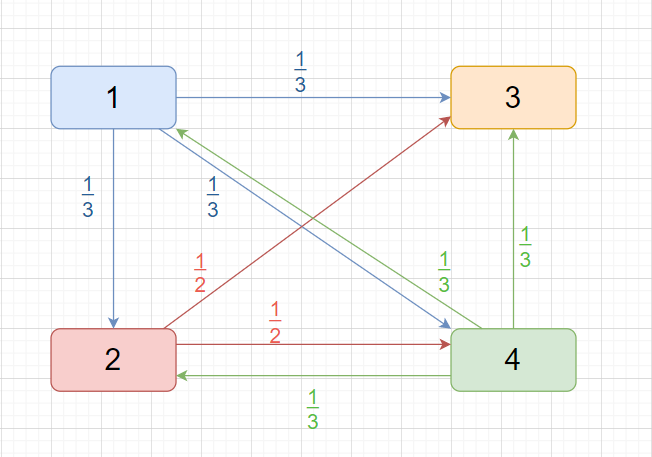
\includegraphics[width=.65\textwidth]{figure/VD1_Dangling Node.png}\end{align}

\begin{itemize}
\item Ta xây dựng được ma trận xác suất chuyển đổi $M$ như sau:\\
            $$ M = 
            \begin{pmatrix}
                %M & 1 & 2 & 3 & 4 \\
                  0 & 0 & 0 & \dfrac{1}{3} \\[10pt]
                \dfrac{1}{3} & 0 & 0 & \dfrac{1}{3} \\[10pt]
                \dfrac{1}{3} & \dfrac{1}{2} & 0 & \dfrac{1}{3} \\[10pt]
                \dfrac{1}{3} & \dfrac{1}{2} & 0 & 0
            \end{pmatrix}
            $$
\item Khởi tạo vector khởi đầu với $(N = 4)$: 
             $$
                 r^{(0)} = \left[\frac{1}{4},\frac{1}{4},\frac{1}{4},\frac{1}{4}\right] ^ T 
            $$
\item Áp dụng phương pháp \emph{Power Iteration} kết quả sau khi lặp nhiều lần là: 
     $$ 
                \begin{pmatrix}
                    r_1 \\[15pt]
                    r_2 \\[15pt]
                    r_3 \\[15pt]
                    r_4 \\[15pt]
                \end{pmatrix}
                =
                \begin{matrix}
                    \dfrac{1}{12} \\[10pt]
                    \dfrac{1}{6} \\[10pt]
                    \dfrac{7}{24}\\[10pt]
                    \dfrac{5}{24} \\[10pt]
                \end{matrix}
                \quad
                \begin{matrix}
                    \dfrac{5}{72} \\[10pt]
                    \dfrac{7}{72} \\[10pt]
                    \dfrac{13}{72}\\[10pt]
                    \dfrac{1}{9} \\[10pt]
                \end{matrix}
                \quad
                \begin{matrix}
                    \dfrac{1}{27} \\[10pt]
                    \dfrac{13}{216} \\[10pt]
                    \dfrac{47}{432}\\[10pt]
                    \dfrac{31}{432} \\[10pt]
                \end{matrix}
                \quad
                \ldots
                \quad
                \begin{matrix}
                    0\\[10pt]
                    0\\[10pt]
                    0\\[10pt]
                    0\\
                \end{matrix}
                $$ 
\end{itemize}
Khi đó, có thể thấy việc xuất hiện \emph{Dangling Node} đã làm cho thuật toán hoạt động sai lệch (node thứ 3 đã hấp thụ các giá trị PageRank mà không thể phân phối chúng) từ đó đưa ra kết quả không đạt yêu cầu tính toán.

%-------------------------------------------------------------------------------
\subsection{Phương án khắc phục}
Phương án khắc phục khi gặp \emph{Dangling Node} là ta sẽ tiến hành chuẩn hóa nó bằng cách thêm \emph{outgoing links} ảo từ \emph{Dangling Node} đến tất cả các node khác có trong \emph{web graph} (kể cả chính nó). 

Giả sử trong \emph{web graph} có $N$ node thì mức độ quan trọng của \emph{Dangling Node}  sẽ được phân phối đều cho $N$ node đó thay vì bị mất. Khi đó, xác suất từ \emph{Dangling Node} truy cập đến các node khác là như nhau và sẽ có giá trị $\dfrac{1}{N}$.

 Sau khi chuẩn hóa \emph{Dangling Node}, \emph{stochastic adjacency matrix} lúc này sẽ được xây dựng trên một công thức chung:\cite{Youtube_Dangling_Node} \\
 
           $$
                M^{'} = M + a^T\left(\dfrac{1}{N} \cdot e\right)
            $$
    Trong đó : 
    \begin{itemize}
        \item $M$ là \textit{stochastic adjacency matrix} ban đầu
        \item $N$ là số lượng node có trong \emph{web graph}
        \item $a$ là ma trận ($n$ x $n$) được xây dựng theo cơ sở:
            \begin{itemize}
                \item Với $i$ là chỉ số dòng, $j$ là chỉ số cột
                \item $a_{ij}=1$ nếu node thứ $i$ không có \emph{outgoing links}, ngược lại $a_{ij}=0$
            \end{itemize}      
        \item $e$ là ma trận đơn vị cấp $n$
   \end{itemize}
    
\textbf{Ví dụ 7:} Chúng ta sẽ tiếp tục sử dụng \emph{web graph} trong ví dụ 6 và bắt đầu thêm \emph{outgoing links} từ node thứ 3 đến các node khác như sau: 1
\begin{align}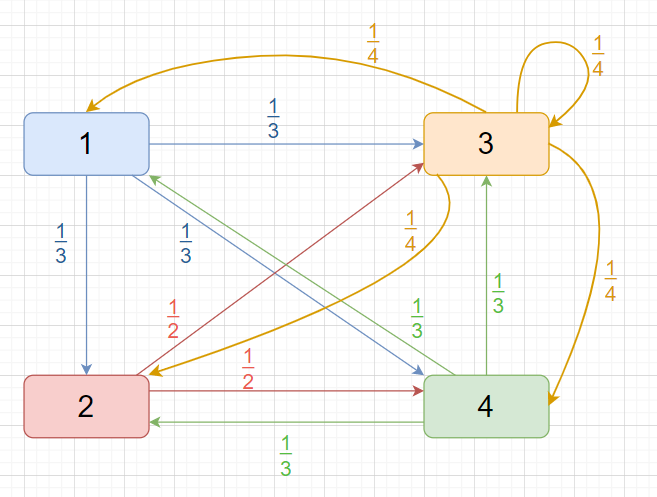
\includegraphics[width=.5\textwidth]{figure/VD2_Dangling Node.png}\end{align}
\begin{itemize}
 
    \item Ta xây dựng được \emph{stochastic adjacency matrix} $M$ là: \\
         $$ M=
        \begin{pmatrix}
            %M & 1 & 2 & 3 & 4 \\
                0 & 0 & \dfrac{1}{4} & \dfrac{1}{3} \\[10pt]
            \dfrac{1}{3} & 0 & \dfrac{1}{4} & \dfrac{1}{3} \\[10pt]
            \dfrac{1}{3} & \dfrac{1}{2} & \dfrac{1}{4} & \dfrac{1}{3} \\[10pt]
            \dfrac{1}{3} & \dfrac{1}{2} & \dfrac{1}{4} & 0
        \end{pmatrix}
        $$
    \item Khởi tạo vector khởi đầu với $(N = 4)$: 
             $$
                 r^{(0)} = \left[\frac{1}{4},\frac{1}{4},\frac{1}{4},\frac{1}{4}\right] ^ T 
            $$
   
    \item Áp dụng phương pháp \emph{Power Iteration} kết quả sau khi lặp nhiều lần là: 
     $$ 
                \begin{pmatrix}
                    r_1 \\[15pt]
                    r_2 \\[15pt]
                    r_3 \\[15pt]
                    r_4 \\[15pt]
                \end{pmatrix}
                =
                \begin{matrix}
                    \dfrac{7}{48} \\[10pt]
                    \dfrac{11}{48} \\[10pt]
                    \dfrac{17}{48}\\[10pt]
                    \dfrac{13}{48} \\[10pt]
                \end{matrix}
                \quad
                \begin{matrix}
                    \dfrac{103}{576} \\[10pt]
                    \dfrac{131}{576} \\[10pt]
                    \dfrac{197}{576}\\[10pt]
                    \dfrac{145}{576} \\[10pt]
                \end{matrix}
                \quad
                \begin{matrix}
                    \dfrac{1171}{6912} \\[10pt]
                    \dfrac{1583}{6912} \\[10pt]
                    \dfrac{2369}{6912}\\[10pt]
                    \dfrac{1789}{6912} \\[10pt]
                \end{matrix}
                \quad
                \ldots
                \quad
                \begin{matrix}
                    \dfrac{6}{35}\\[10pt]
                    \dfrac{8}{35}\\[10pt]
                    \dfrac{12}{35}\\[10pt]
                    \dfrac{9}{35}\\
                \end{matrix}
                $$ 
\end{itemize}
Như vậy chúng ta đã khắc phục được vấn đề \emph{Dangling Node}.
%------------------------------------------------------------------------------------
\section{Web reducible}
\subsection{Đặt vấn đề}
 Đây là trường hợp khi \emph{web graph} không phải là một \emph{đồ thị liên thông mạnh}, khi đó \emph{web graph} sẽ gồm nhiều thành phần liên thông khác nhau. Từ đó, khi duyệt qua đồ thị thì từ một node ở thành phần liên thông này có thể không truy cập được đến một node của thành phần liên thông khác. Điều này dẫn đến việc giá trị PageRank của các trang này không được tính toán chính xác. Khi đó đồ thị sẽ mang tính chất \emph{reducible}.\\
 
 \textbf{Ví dụ 8}: \emph{Web graph} sau đây là một \emph{reducible graph}.
 \begin{align}
                 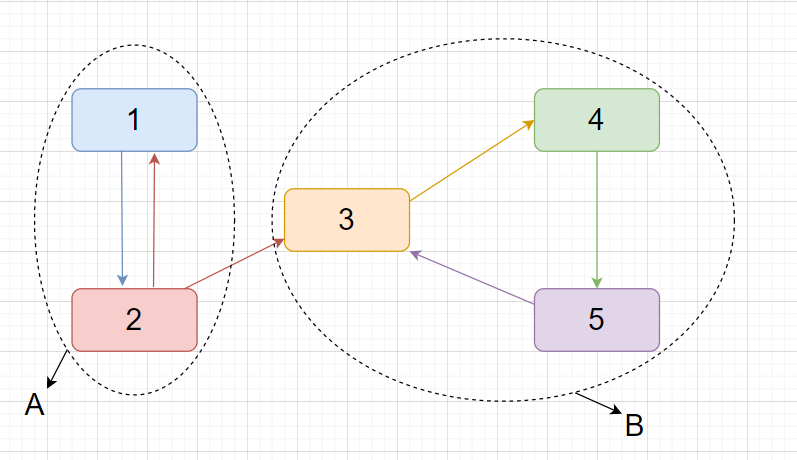
\includegraphics[width=.5\textwidth]{figure/VD1_Web Reducible.png}
            \end{align}

Chúng ta sẽ thử áp dụng phương pháp \emph{Power Iteration} để đi tìm \emph{rank vector} cho ví dụ trên như sau:\\
\begin{itemize}
     \item Ta xây dựng được \emph{stochastic adjacency matrix} $M$ là:
     $$ M = 
            \begin{pmatrix}
                %M & 1 & 2 & 3 & 4 \\
                  0 & \dfrac{1}{2} & 0 & 0 & 0 \\[10pt]
                1 & 0 & 0 & 0 & 0 \\[10pt]
                0 & \dfrac{1}{2} & 0 & 0 & 1 \\[10pt]
                0 & 0 & 1 & 0 & 0 \\[10pt]
                0 & 0 & 0 & 1 & 0
            \end{pmatrix}
    $$
    \item Với vector khởi đầu với $(N = 5)$: 
             $$
                        r^{(0)} = \left[\frac{1}{5},\frac{1}{5},\frac{1}{5},\frac{1}{5},\frac{1}{5}\right] ^ T 
            $$
    \item Ta được kết quả sau khi lặp nhiều lần như sau: \\
                $$
                \begin{pmatrix}
                    r_1 \\[15pt]
                    r_2 \\[15pt]
                    r_3 \\[15pt]
                    r_4 \\[15pt]
                    r_5 
                \end{pmatrix}
                =
                \begin{matrix}
                    \dfrac{1}{10} \\[10pt]
                    \dfrac{1}{5} \\[10pt]
                    \dfrac{3}{10}\\[10pt]
                    \dfrac{1}{5} \\[10pt]
                    \dfrac{1}{5}
                \end{matrix}
                \quad
                \begin{matrix}
                    \dfrac{1}{10} \\[10pt]
                    \dfrac{1}{10} \\[10pt]
                    \dfrac{3}{10}\\[10pt]
                    \dfrac{3}{10} \\[10pt]
                    \dfrac{1}{5}
                \end{matrix}
                \quad
                \begin{matrix}
                    \dfrac{1}{20} \\[10pt]
                    \dfrac{1}{10} \\[10pt]
                    \dfrac{1}{4}\\[10pt]
                    \dfrac{3}{10} \\[10pt]
                    \dfrac{3}{10}
                \end{matrix}
                \quad
                \ldots
                \quad
                \begin{matrix}
                    0 \\[10pt]
                    0 \\[10pt]
                    \dfrac{12}{35}\\[10pt]
                    \dfrac{13}{35} \\[10pt]
                    \dfrac{2}{7}
                \end{matrix}
                $$ 
    \item Quá trình tìm \emph{rank vector} cho ra kết quả là một vector có chứa phần tử mang giá trị bằng 0 tức là sẽ tồn tại trang web có chỉ số PageRank bằng 0. Điều này là vô lý, do đó kết quả trên quả trên là sai. Vậy sẽ không tìm được chính xác PageRank của trang web. 
\end{itemize}

\textbf{Ví dụ 9:}
\begin{align}
                 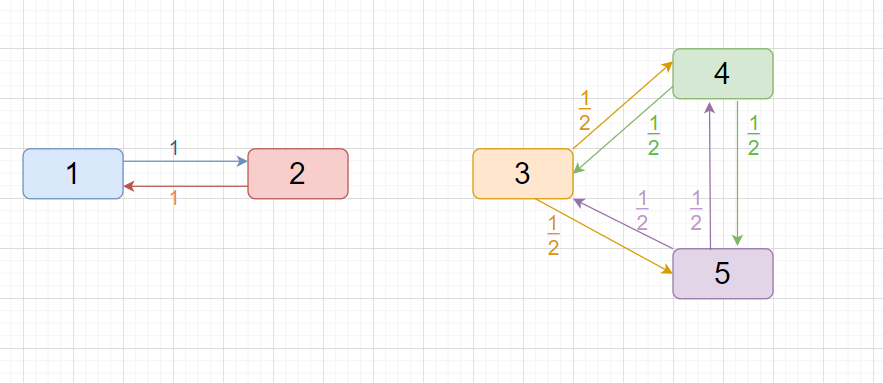
\includegraphics[width=.65\textwidth]{figure/VD2_Web Reducible.png}
            \end{align}
\begin{itemize}
    \item Ta xây dựng được \emph{stochastic adjacency matrix} $M$ cho \emph{web graph} trên như sau: 
     $$ M =
            \begin{pmatrix}
                %M & 1 & 2 & 3 & 4 \\
                  0 & 1& 0 & 0 & 0 \\[10pt]
                1 & 0 & 0 & 0 & 0 \\[10pt]
                0 & 0 & 0 & \dfrac{1}{2} & \dfrac{1}{2} \\[10pt]
                0 & 0 & \dfrac{1}{2} & 0 & \dfrac{1}{2} \\[10pt]
                0 & 0 & \dfrac{1}{2}& \dfrac{1}{2} & 0
            \end{pmatrix}
    $$
    \item Ứng với trị riêng bằng 1 ta tìm được hai \emph{vector riêng} của ma trận M là :\\ $ v = \begin{pmatrix}
                    1 \\
                    1 \\
                    0\\
                    0\\
                    0
                \end{pmatrix}
                \text{và } u = \begin{pmatrix}
                    0\\
                    0\\
                    1\\
                    1\\
                    1
                \end{pmatrix} $ 
    \item Tuy nhiên hai \emph{vector riêng} này độc lập với nhau nên dẫn đến sẽ có hai \emph{rank vector} cho một \emph{web graph}. Điều này là vô lý.
\end{itemize}

Từ hai ví dụ trên cho thấy các trường hợp \emph{reducible graph} thì đều không thể tìm được PageRank chính xác cho trang web nên chúng ta cần phải đưa ra hướng khắc phục.
\subsection{Phương án khắc phục}
Với mỗi bước, mô hình \textit{random surfer} sẽ có 2 lựa chọn: 
\begin{itemize}
    \item Với xác suất $\beta$, theo một liên kết đến 1 trang web ngẫu nhiên như bình thường.
    \item Với xác suất $1-\beta$, nhảy đến 1 trang bất kỳ .
\end{itemize}
Giá trị $\beta$ đã được ước lượng sẽ có giá trị từ $0.8 \rightarrow 0.9$. Điều đó tương đương với việc mô hình \textit{random surfer} sẽ chọn một liên kết ngẫu nhiên 5 lần sau đó nhảy đến trang bất kì 1 lần.\\[10pt]
\textbf{Ta có phương trình:}
$$r_j = \sum_{i \rightarrow j}\beta\dfrac{r_i}{d_i} + (1-\beta)\dfrac{1}{N}$$
\textbf{Ma trận tương ứng:}
$$ A = \beta M + (1 - \beta) \left[\dfrac{1}{N}\right]_{N\text{x}N} $$
Chúng ta sẽ dùng phương pháp luỹ thừa và tìm ra phân phối xác suất cố định $r$ qua phương trình: 
$$r=Ar$$
\textbf{Ví dụ 10:} Dựa vào phương pháp trên ta sẽ tính PageRank cho \textit{web graph} ở ví dụ 8 với $\beta = 0.85$.
     $$ M = 
            \begin{pmatrix}
                %M & 1 & 2 & 3 & 4 \\
                  0 & \dfrac{1}{2} & 0 & 0 & 0 \\[10pt]
                1 & 0 & 0 & 0 & 0 \\[10pt]
                0 & \dfrac{1}{2} & 0 & 0 & 1 \\[10pt]
                0 & 0 & 1 & 0 & 0 \\[10pt]
                0 & 0 & 0 & 1 & 0.
            \end{pmatrix}
    $$

$$
A = 0.85 
            \begin{pmatrix}
                 0 & \dfrac{1}{2} & 0 & 0 & 0 \\[10pt]
                1 & 0 & 0 & 0 & 0 \\[10pt]
                0 & \dfrac{1}{2} & 0 & 0 & 1 \\[10pt]
                0 & 0 & 1 & 0 & 0 \\[10pt]
                0 & 0 & 0 & 1 & 0
            \end{pmatrix}
            + (1 - 0.85 )  
             \begin{pmatrix}
                \dfrac{1}{5} & \dfrac{1}{5}& \dfrac{1}{5} & \dfrac{1}{5} & \dfrac{1}{5} \\[10pt]
                \dfrac{1}{5} & \dfrac{1}{5} & \dfrac{1}{5} & \dfrac{1}{5} & \dfrac{1}{5} \\[10pt]
                \dfrac{1}{5} & \dfrac{1}{5} & \dfrac{1}{5} & \dfrac{1}{5} & \dfrac{1}{5} \\[10pt]
                \dfrac{1}{5} & \dfrac{1}{5} & \dfrac{1}{5} & \dfrac{1}{5} & \dfrac{1}{5} \\[10pt]
                \dfrac{1}{5} & \dfrac{1}{5} & \dfrac{1}{5} & \dfrac{1}{5} & \dfrac{1}{5} \\[10pt]
            \end{pmatrix}
            =
            \begin{pmatrix}
                \dfrac{3}{100} & \dfrac{91}{200}& \dfrac{3}{100} & \dfrac{3}{100} & \dfrac{3}{100} \\[10pt]
                \dfrac{22}{25} & \dfrac{3}{100} & \dfrac{3}{100} & \dfrac{3}{100} & \dfrac{3}{100} \\[10pt]
                \dfrac{3}{100} & \dfrac{91}{200} & \dfrac{3}{100} & \dfrac{3}{100} & \dfrac{22}{25} \\[10pt]
                \dfrac{3}{100} & \dfrac{3}{100} & \dfrac{22}{25} & \dfrac{3}{100} & \dfrac{3}{100} \\[10pt]
                \dfrac{3}{100} & \dfrac{3}{100} & \dfrac{3}{100} & \dfrac{22}{25} & \dfrac{3}{100} \\[10pt] 
            \end{pmatrix}
$$

Với vector khởi đầu với $(N = 5)$: 
             $$
                        r^{(0)} = \left[\frac{1}{5},\frac{1}{5},\frac{1}{5},\frac{1}{5},\frac{1}{5}\right] ^ T 
            $$
            
Ta được kết quả sau khi lặp nhiều lần như sau: \\
                $$
                \begin{pmatrix}
                    r_1 \\[15pt]
                    r_2 \\[15pt]
                    r_3 \\[15pt]
                    r_4 \\[15pt]
                    r_5 
                \end{pmatrix}
                =
                \begin{matrix}
                    \dfrac{23}{200} \\[10pt]
                    \dfrac{1}{5} \\[10pt]
                    \dfrac{57}{200}\\[10pt]
                    \dfrac{1}{5} \\[10pt]
                    \dfrac{1}{5}
                \end{matrix}
                \quad
                \begin{matrix}
                    \dfrac{23}{200} \\[10pt]
                    \dfrac{511}{4000} \\[10pt]
                    \dfrac{57}{200}\\[10pt]
                    \dfrac{1089}{4000} \\[10pt]
                    \dfrac{1}{5}
                \end{matrix}
                \quad
                \ldots
                \quad
                \begin{matrix}
                    \dfrac{171}{2555} \\[10pt]
                    \dfrac{222}{2555} \\[10pt]
                    \dfrac{777419}{2629095} \\[10pt]
                    \dfrac{739679}{2629095} \\[10pt]
                    \dfrac{141520}{525819}
                \end{matrix}
                $$